\documentclass[a4paper,12pt]{article}
\usepackage[english,activeacute]{babel}
\usepackage[ansinew]{inputenc}
\usepackage[T1]{fontenc}
\usepackage{amsmath,amsfonts,amssymb}
\usepackage{graphicx}
\usepackage{titlesec}
\usepackage{longtable}
\usepackage{dsfont}
\usepackage{wrapfig}
\usepackage{hyperref}
\usepackage{cancel}
\usepackage{epigraph}
\usepackage{appendix}
\usepackage{marvosym}
\usepackage{enumerate} %For enumerating with letters with option [a)]
\usepackage{fancyvrb} %To reduce font size in verbatim environment
\usepackage{epstopdf}
\usepackage{color}
\usepackage[flushleft]{threeparttable}
\usepackage{natbib}
\usepackage{subfig}
%\usepackage{subcaption}
\usepackage{etoolbox}
\usepackage{array}
\usepackage{booktabs}
\usepackage[super]{nth}
\usepackage{breqn} %Breaks equations automatically
\usepackage{float}

\setlength\epigraphwidth{10cm}
\setlength\epigraphrule{0pt}
\newcolumntype{P}[1]{>{\centering\arraybackslash}p{#1}}


\newtheorem{definition}{Definition}
\newtheorem{proposition}{Proposition}
\newtheorem{theorem}{Theorem}
\newtheorem{corollary}{Corollary}

% === To embed exercises within the notes === %
\newtheorem{exercise}{Exercise}

\newcommand{\ts}{\textsuperscript}
\newcommand{\source}[1]{\caption*{\tiny Source: {#1}} }
\DeclareMathOperator{\sgn}{sgn}

\usepackage[left=2cm,right=2cm,top=2cm,bottom=2cm]{geometry}


\title{\textbf{QED Macroeconomics III: Problem Set Matlab 2}}

\author{Rafael Serrano Quintero
\thanks{Department of Fundamentos del An{\'a}lisis Econ{\'o}mico, Universidad de Alicante. Email: \texttt{r.serrano@ua.es}} \\
Universidad de Alicante \\}
\date{}


\begin{document}
\maketitle

\textbf{The due date for this Problem Set is Tuesday \nth{24} April 2018 before the class.} 

\begin{exercise}
Chaotic dynamics. The dynamics of the following function can become chaotic for some values of $\rho$.
	 \[
	 x_{t+1} = \rho x_t (1-x_t)
	 \]

\begin{enumerate}[a)]
		 \item Let's create a function \texttt{chaos} that returns the sequence $\{x_t\}_{t=0}^{T}$ for a given initial condition $x_0\in [0,1]$, a parameter $\rho\in [0,4]$, and a simulation length $T$. The function should display an error if the initial condition is not in those bounds or if the parameter is not in those bounds, the error should say \textit{which case happened}.
	 	 \item Use your function \texttt{chaos} to plot a \textbf{bifurcation diagram}. This is a diagram that plots the dynamics of the series for different values of $\rho$ with the same initial condition. The logic of the algorithm should be something like:	 
	 	 \begin{itemize}
		 	\item Simulate the dynamics using the function with an initial condition. Make a long simulation (around $1000$ periods).
	 		\item Discard all observations but the last $50$.
	 		\item Plot in the $x$ axis the value for $\rho$ and in the $y$ axis the values of the series. To do this, it is convenient (but not necessary) to use a \texttt{while} loop. Start with a value for $\rho$ of $2.5$. \underline{Hint:} notice that the plot command that displays the bifurcation diagram should be inside the loop, \href{https://www.mathworks.com/matlabcentral/answers/90680-plotting-in-a-for-loop}{\textcolor{blue}{check Matlab forums}}!. The result should be something like Figure \ref{bifurc}. 
	 	\end{itemize}
\end{enumerate}

\begin{figure}[htbp]
	\centering
		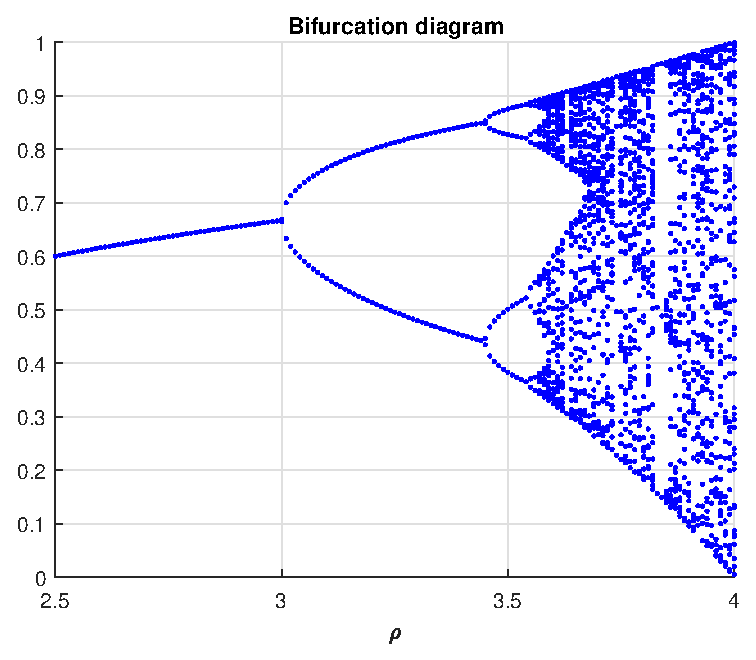
\includegraphics[width=0.55\textwidth]{bifurc.eps}
	\caption{Bifurcation Diagram}
	\label{bifurc}
\end{figure}
\end{exercise}


\begin{exercise}
Simulate variables and perform a linear regression with OLS. Suppose you have a model like:
	
\[
y_t = \beta_1 + \beta_2 x_{2t} +\beta_3 x_{3t} +\varepsilon_t
\]
	
Where $x_2$ is a trend variable that takes values $(1,2,3,\ldots,T)$ plus an iid shock $u_t\thicksim \mathcal{N}(0,\sigma_u)$. $x_3$ is a random variable uniformly distributed in $[3, 5]$, and $\varepsilon$ is an iid normally distributed error term with mean 0 and standard deviation $\sigma_{\varepsilon}$. Simulate the explanatory variables and the dependent variable following the model, perform OLS, and plot the residuals. Assume that the true parameter values are:
	
\[
\beta_1 = 5, \beta_2 = 1, \beta_3 = 0.1, \sigma_e = 0.04, \sigma_u = 0.02
\]

Simulate $100$ observations of each variable. \underline{Hint:} try not to use loops, they are not necessary in this exercise. Do not use built-in functions to estimate the coefficients, you should program the estimator. It is enough to compute just the $\hat{\beta}$.
\end{exercise}

\begin{exercise}

\textbf{Taken from Quant-Econ.}

Suppose that a worker at any point in time can be at one of two possible states, unemployed (state 1) or employed (state 2). For an unemployed worker, the probability of getting a job is $\alpha\in(0,1)$, while for an employed worker, the probability of going unemployed is $\beta\in(0,1)$. We can define a stochastic matrix $\mathbf{P}$ so that each entry gives us the probability of changing from one state to another. So if, $\mathbf{P}(1,2) = \alpha$ and $\mathbf{P}(2,1) = \beta$, the stochastic matrix is:

\[
\mathbf{P} = \begin{bmatrix}
1-\alpha & \alpha \\
\beta & 1-\beta
\end{bmatrix}
\]
	
This is an example of a \textbf{Markov Chain}. Under some conditions (aperiodicity and irreducibility; you will see that in some other courses), we can define what is called as the \textbf{stationary distribution} $\psi^* = \psi^* \mathbf{P}$ where $\psi^* = (p, 1-p)$ and, by ergodicity, $p$ is approximately the fraction of time a worker will remain unemployed $p = \frac{\beta}{\alpha + \beta}$ (somewhat like a steady state). What makes this a Markov chain is that it satisfies the Markov property, that is, $\{X_t\}$ is a Markov chain on $\mathcal{S}$ where $\mathcal{S}$ is the set of states if for any date $t$ and any state $s'\in \mathcal{S}$:

\[
\mathbb{P}\{X_{t+1} = s' | X_t\} = \mathbb{P}\{X_{t+1} = s' | X_t, X_{t-1},\ldots\}
\]
	
That is the same as to say that the current state summarizes all information needed to compute the probability of being in a particular state in the next period. In particular, the dynamics of a Markov chain are fully determined by the set of values:
	
\[
\mathbf{P}[s,s'] := \mathbb{P}\{X_{t+1} = s' | X_t = s\} \ (s,s'\in\mathcal{S})
\]
	
There's a theorem that tells us that if the conditions above mentioned are satisfied (aperiodicity and irreducibility) by $\mathbf{P}$, then $\mathbf{P}$ has exactly one stationary distribution $\psi^*$ and that, for any initial distribution $\psi_0$, we have that $\left\lVert \psi_0 \mathbf{P}^t - \psi^* \right\rVert\rightarrow 0$ as $t\rightarrow\infty$. That means that as we increase the periods, we will converge to the stationary distribution.
	
In this exercise, you need to create a function \texttt{markov_chain} that takes as inputs a stochastic matrix $\mathbf{P}$, an initial state $x_0$, the length of the simulation $T$, and the number of possible states. What we will also need is an initial state (or a probability distribution for the initial state to be drawn from). So the Markov Chain will be constructed:

\begin{enumerate}
	\item At time $t=0$, $X_0$ is set to an initial state.
	\item At each subsequent time $t$, $X_{t+1}$ will be drawn from $\mathbf{P}[X_t,\cdot]$.
\end{enumerate}
	
The function should return the sequence for $\{X_t\}$. Start by declaring the first point of the sequence (the initial state). Then use a \texttt{for} loop. Here you have a pseudo-code of what is asked. 

\begin{Verbatim}[numbers = left]
function [Markov Path] = markov_chain(P,x0,T,states)
	1st Markov Path = x0
	for time = 2 to T
		psi = P(previous state of X,:)
		Markov Path in t = Random sample from the psi distribution 
		of one of the two possible states.
	end
end
\end{Verbatim}

For the random sampling, check the command \texttt{randsample}. Set the option replacement to be true. Test the function by taking $2$ states, setting probabilities $\alpha = 1/3$ and $\beta = 1/4$, choose $30$ periods and assume you start in state $1$.
\end{exercise}


\begin{exercise}
To test our function \texttt{markov_chain}, we will use the unemployment model described above. Set $\alpha = \beta = 0.25$ and a long simulation ($\approx 3000$ periods). What we will do is to simulate two Markov chains with this model, one with an initial state unemployed ($x_0 = 1$), and another with initial state employed ($x_0 = 2$). First, simulate the Markov chain for both cases using the function created in previous exercise. Second, we want to check whether the fraction of time spent unemployed converges to the stationary distribution. To do so, we will want to compute:

\[
\bar{X}_n = \frac{1}{n} \sum^n_{t=1} \mathbf{1}\{X_t = 1\}
\]
	
Where $\mathbf{1}\{X_t = 1\}$ is an indicator function that takes value equal to one if $X_t = 1$. That is, we want to compute the average time a worker spent unemployed at each $t$. To compute this, first create a for loop that iterates over all periods of time $(1...T)$. Inside that loop, create a conditional (boolean) expression that tells us whether at that moment the series for the initial condition $X_0=1$ took actually the value one, if that happened, create an index that puts a $1$ in that observation and a $0$ otherwise. Do the same for the series with initial condition $X_0 = 2$. The pseudo-code I used is something like:

\begin{Verbatim}[numbers = left]
Declare parameters:
alpha, beta, T, p from the stationary distribution, 
the stochastic matrix, and the two initial states

Construct the two Markov Chains using the function:
	Markov Chain 1 = Start Unemployed
	Markov Chain 2 = Start Employed

for t = 1 to T
	if at t, the started unemployed is unemployed
		Set the index for starting unemployed at t as 1
	Otherwise
		Set the index for starting unemployed at t as 0
	end
	
	For the starting employed series do the same
end
\end{Verbatim}

Once you have done this, create a column vector from $1$ to $T$ and compute the cumulative sum of the indexes created before divided by this index to obtain $\bar{X}_n$ (you should obtain two $\bar{X}_n$, one for each series with different initial conditions). Finally, plot in the $x$ axis the vector from $1$ to $T$ and, in the $y$ axis, $\bar{X}_n - p$ for the two series with different initial conditions. The result should be something like Figure \ref{unemployment_dynamics}.
	
\begin{figure}[htbp]
\centering
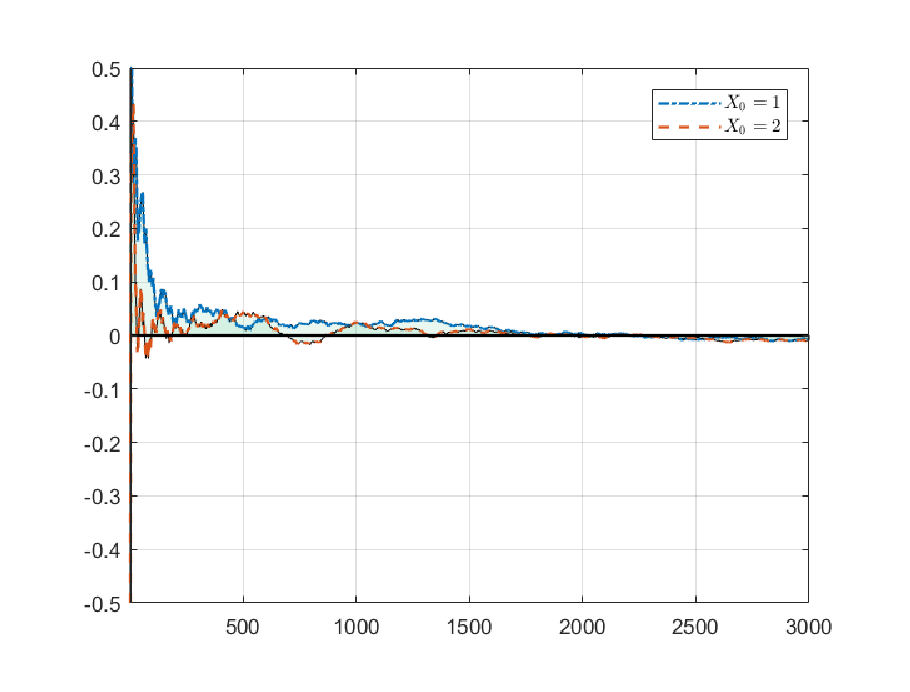
\includegraphics[width = 0.65\textwidth]{unemployment_dynamics.eps}
\caption{Convergence to Stationary Distribution}
\label{unemployment_dynamics}
\end{figure}
\end{exercise}

\begin{exercise}
Fitting the GDP. First, download the series for GDP per capita in quarterly basis from the Federal Reserve Bank of St. Louis (you can download them from \href{https://fred.stlouisfed.org/series/A939RX0Q048SBEA}{\textcolor{blue}{\textbf{here}}}). The purpose of this exercise is that you familiarize yourself with extracting data from files and manipulate it in Matlab. Start this exercise in a new script, start by clearing the workspace and the command window.

\begin{enumerate}
	\item As a zero step, input the data as a variable called $Y_t$, and take the length of the series as a variable $T$. Compute also the growth rate of GDP per capita in this step and save it as another variable, for example $g_Y$.
	\item First, suppose we want to just fit a time trend. To do so, suppose the model we have for the evolution of output is:
	\begin{equation}
	Y_t = e^{\phi_1 t + \phi_2} + \varepsilon_t \ ; \ \varepsilon_t \underset{iid}{\thicksim} \mathcal{N}(0,\sigma^2_{\varepsilon})
	\label{model_1}
	\end{equation}
		
Where $t$ is a time trend, $\phi_1$ and $\phi_2$ are the parameters of interest, and $\varepsilon$ is white noise. Your task is to estimate parameters $\phi_1$ and $\phi_2$ using \texttt{lsqcurvefit}. For the initial values, take $\phi_2 = 1$, and for $\phi_1$ one that you believe makes sense, and explain why. Plot the data, and the fitted curve. The result should be something like Figure \ref{exp_fit}.
		
\begin{figure}[htbp]
	\centering
		\includegraphics[width = 0.65\textwidth]{exp_fit.eps}
	\caption{Exponential Fit of GDP per capita}
	\label{exp_fit}
\end{figure} 

	\item Let us now take a different approach, we will try to fit the \textbf{growth rate} of GDP per capita, which is stationary, using an $AR(2)$ specification\footnote{Please, take into account this is an exercise, this is not a good way to forecast GDP nor almost any economic variable. We should \textit{at least} use a VAR specification, but this is a good exercise to familiarize yourself with estimation methods in Matlab.}. 
	
		\begin{equation}
		g_{Y,t} = \alpha + \rho_1 g_{Y,t-1} + \rho_2 g_{Y,t-2} + u_t \ ; \ u_t \underset{iid}{\thicksim} \mathcal{N}(0, \sigma^2_u)
		\label{model_2}
		\end{equation}
		
	Where $\alpha$ is a constant, $\rho_1$ and $\rho_2$ are the autoregressive parameters of the model, and $u_t$ is white noise. Estimate this model via OLS. The estimator should be programmed \textbf{by yourselves}, do not use built-in functions or user-defined functions. Obtain the parameters $\rho_1$, $\rho_2$, an estimate of $\hat{\sigma}^2_u$, and the variance-covariance matrix of the OLS estimator. Recall that:
		
		\begin{align}
		\mathbb{E}\left[(\hat{\rho}-\rho)(\hat{\rho}-\rho)'\right] &= \sigma^2\left(X'X\right)^{-1} \label{varcovOLS}\\
		\hat{\sigma}^2 &= \frac{\hat{u}' \hat{u}}{n-k} \label{sigmahat}
		\end{align}
		
	Where $(n-k)$ denotes the degrees of freedom, \eqref{varcovOLS} gives the Variance-Covariance Matrix for the OLS estimator, and \eqref{sigmahat} is the estimator for the variance of the residuals with $k$ the number of regressors.
	
	\item Under Normality, OLS and Maximum Likelihood are equivalent. Let's check that by estimating the model in \eqref{model_2} and compare our results. We can proceed as:
	\begin{enumerate}
		\item Create a vector of initial values for $\alpha$, $\rho_1$, $\rho_2$, and $\sigma_u$, use the values $\tilde{\rho} = \left[1 , \ 0.5 , \ 0.5, \  0.2\right]$.
		\item Construct a function \texttt{my_mle} that takes as inputs a vector of coefficients and the data matrix, and returns the sum of the log-likelihood across observations. Recall that the likelihood takes the form:
		\[
		\mathcal{L}(\rho) = \left(2\pi \sigma_u^2\right)^{-T/2} exp\left(-\frac{1}{2\sigma_u^2}\sum^T_{i=1} \left(g_{Y,i} - \hat{g}_{Y,i} \right)^2\right)
		\]
		\item Find parameter estimates and the likelihood using \texttt{fminunc}.	
	\end{enumerate}
	
	Plot the predicted values for the OLS estimates, the MLE estimates, and the data for comparison. Clarify which series is which in a legend.
\end{enumerate}
\end{exercise}


\end{document}